\documentclass{article}
\usepackage[final]{nips_2017}
\usepackage[utf8]{inputenc} % allow utf-8 input
\usepackage[T1]{fontenc}    % use 8-bit T1 fonts
\usepackage{hyperref}       % hyperlinks
\usepackage{url}            % simple URL typesetting
\usepackage{booktabs}       % professional-quality tables
\usepackage{amsfonts}       % blackboard math symbols
\usepackage{nicefrac}       % compact symbols for 1/2, etc.
\usepackage{microtype}      % microtypography
\usepackage{graphicx}
\title{Family kinship Recognition Using Deep Learning}

\author{
  Bruce Jianye Liu\thanks{personal github profile
    https://github.com/brucelau-github\\
  Department of Computer Science\\
  Stanford University\\
  \texttt{bruceliu@stanford.edu} \\
  %% examples of more authors
  %% \And
  %% Coauthor \\
  %% Affiliation \\
  %% Address \\
  %% \texttt{email} \\
  %% \AND
  %% Coauthor \\
  %% Affiliation \\
  %% Address \\
  %% \texttt{email} \\
  %% \And
  %% Coauthor \\
  %% Affiliation \\
  %% Address \\
  %% \texttt{email} \\
  %% \And
  %% Coauthor \\
  %% Affiliation \\
  %% Address \\
  %% \texttt{email} \\
}

\begin{document}
% \nipsfinalcopy is no longer used

\begin{center}
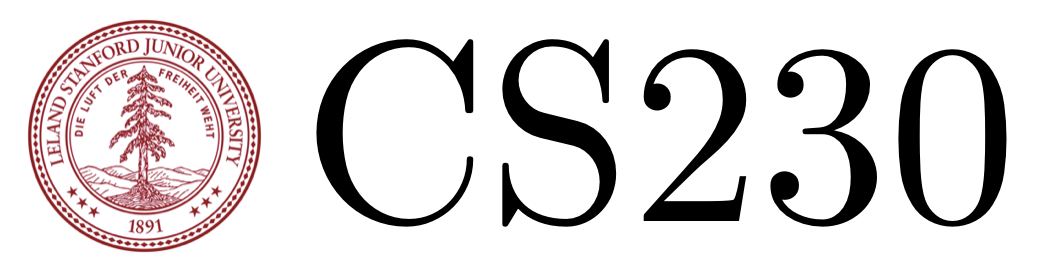
\includegraphics[width=3cm, height=0.7cm]{CS230}
\end{center}

\maketitle

\begin{abstract}
Family kin is an easy task for human. missing children, missing parent, silbling searching, share photos, kinship verification, DNA privacy. Face recoginition develop very well. A approach to find parents.
\end{abstract}

\section{Introduction}
working on it.

\section{Related work}
working on it.

\section{Dataset and Features}
working on it.


\section{ Methods }
working on it.

\section{Experiments/Results/Discussion}
working on it.

\section{Conclusion/Future Work }

\section{Contributions}

\section*{References}
\medskip
\small
[1] Alexander, J.A.\ \& Mozer, M.C.\ (1995) Template-based algorithms
for connectionist rule extraction. In G.\ Tesauro, D.S.\ Touretzky and
T.K.\ Leen (eds.), {\it Advances in Neural Information Processing
  Systems 7}, pp.\ 609--616. Cambridge, MA: MIT Press.

\end{document}
